\chapter{Geometry and groups}
\label{ch:euclidean}
%% \section{euclidean frames, relation to determinants(?)}
%% \section{the euclidean group as a semidirect product}
%% \section{euclidean properties (length, angle, etc.)}


In this chapter we study Euclidean geometry.  We assume some standard linear
algebra over real numbers, including the notion of finite dimensional vector
space over the real numbers and the notion of inner product.  In our context,
the field of real numbers, $\RR$, is a set, and so are vector spaces over it.
Moreover, a vector space $V$ has an underlying additive abstract group, and we
will feel free to pass from it to the corresponding group.

\section{Inner product spaces}

\begin{definition}\label{def:InnerProductSpace}
  An {\em inner product space} $V$ is a real vector space of finite dimension
  equipped with an inner product $H : V \times V \to \RR $.
\end{definition}

Let $\OS$ denote the type of inner product spaces.  It is a type of pairs whose
elements are of the form $(V,H)$.
For $n : \NN$, let $\OS_n$ denote the type of inner product spaces of dimension $n$.

For each natural number $n$, we may construct the {\em standard} inner product
space $\VV^n \defeq (V,H)$ of dimension $n$ as follows.  For $V$ we take the
vector space $\RR^n$, and we equip it with the standard inner product given by
the dot product
$$ H ( x , y) \defeq x \cdot y, $$
where the dot product is defined as usual as
$$ x \cdot y \defeq \sum_i x_i y_i . $$

\begin{theorem}\label{thm:GramSchmidt}
  Any inner product space $V$ is merely equal to $\VV^n$, where $n$ is $\dim V$.
\end{theorem}

For the definition of the adverb ``merely'', refer to \cref{def:merely}.

\begin{proof}
  Since any finite dimensional vector space merely has a basis, we may assume
  we have a basis for $V$.  Now use Gram-Schmidt orthonormalization to show
  that $V = \VV^n$.
\end{proof}

\begin{lemma}\label{lem:InnerProductSpace1Type}
  The type $\OS$ is a $1$-type.
\end{lemma}

\begin{proof}
  Given two inner product spaces $V$ and $V'$, we must show that the type
  $V=V'$ is a set.  By univalence, its elements correspond to the linear
  isomorphisms $f : V \xrightarrow \weq V'$ that are compatible with the
  inner products.  Those form a set.
\end{proof}

\begin{definition}\label{def:OrthogonalGroup}
  Given a natural number $n$, we define the {\em orthogonal group} $\OrthGp n$
  as follows.
  $$\OrthGp n \defeq \mkgroup \OS_n$$
  Here $\OS_n$ is equipped with the basepoint provided by $\shape_{\OrthGp n} \defeq \VV^n$, and with the
  proof that it is a connected groupoid provided by \cref{thm:GramSchmidt} and
  \cref{lem:InnerProductSpace1Type}.
\end{definition}

The standard action (in the sense of \cref{std-action}) of $\OrthGp n$ is an
action of it on its designated shape $\VV^n$.  Letting $\typeRealVectorSpace$ denote
the type of finite dimensional real vector spaces, we may compose the standard
action with the projection map $\B \OrthGp n \to \typeRealVectorSpace$ that
forgets the inner product to get an action of $\OrthGp n$ on the vector space
$\RR^n$.

\section{Euclidean spaces}

In high school geometry courses, one encounters the Euclidean plane (of
dimension 2) and the Euclidean space of dimension 3.  The vectors and the
points of Euclidean geometry are the basic ingredients, from which the other
concepts are derived.  Those concepts include such things as lines, line
segments, triangles, tetrahedra, spheres, and so on.  Symmetries of those
objects are also studied: for example, an isosceles non-equilateral triangle has
a total of 2 symmetries: the identity and the reflection through the midline.

So, a Euclidean space will come with two sets: a set of points and a set of
vectors.  The structure on the two sets includes the following items.

\begin{enumerate}
\item If $v$ and $w$ are vectors, then there is a vector $v+w$ called its {\em
  sum}.
\item If $v$ is a vector and $r$ is a real number, then there is a vector $rv$
  called the {\em scalar multiple} of $v$ by $r$.
\item If $v$ is a vector, then there is a real nonnegative number called its
  {\em length}.
\item If $P$ and $Q$ are points, then
  there is a unique vector $v$ which can be ``positioned'' so its tail is ``at''
  $P$ and its head is ``at'' $Q$.  It is called the vector {\em from $P$ to
    $Q$}.  The {\em distance} from $P$ to $Q$ is the length of $v$.  
\item If $P$ is a point and $v$ is a vector, then there is a unique point $Q$
  so that $v$ which can be positioned so its tail is at
  $P$ and its head is at $Q$.  It is called the point obtained from $P$ by {\em
    translation along $v$.}
\end{enumerate}

We introduce the (new) notation $v+P$ for the point $Q$ obtained from $P$ by
translation along $v$.  Another fact from high school geometry is that if $w$
is a vector, too, then the associative rule $v+(w+P) = (v+w)+P$ holds.  This
suggests that the essential features of high school geometry can be captured by
describing the set of points as a torsor for the group of vectors.

We use that idea now to give a precise definition of {\em Euclidean space of
  dimension $n$}, together with its points and vectors.  More complicated
geometric objects will be introduced in subsequent sections.

\begin{definition}\label{def:EuclideanSpace}
  A {\em Euclidean space} $E$ is an torsor $A$ for the additive group
  underlying an inner product space $V$.  (For the definition of torsor, see
  \cref{def:abstrGtorsors}.)
\end{definition}

We will write $V$ also for the additive group underlying $V$.  Thus an
expression such as $\B V$ or $\typetorsor_V$ will be understood as applying to
the underlying additive group\footnote{We are careful not to refer to the group
  as an Abelian group at this point, even though it is one, because the
  operator $\B$ may be used in some contexts to denote a different construction
  on Abelian groups.}
of $V$.

\begin{definition}
  We denote the type of all Euclidean spaces of dimension $n$ by $\ES_n \defeq
  \sum_{V:\OS_n} \typetorsor_V$.  The elements of $\Points E$ will be the {\em
    points} in the geometry of $E$, and the elements of $\Vectors E$ will be the
      {\em vectors} in the geometry of $E$.
      We let $\ES$ denote the type of all Euclidean spaces; it is equivalent to the
      sum $\sum_{n:\NN} \ES_n$.
\end{definition}

The torsor $\Points E$ is a nonempty set upon which $V$ acts.  Since $V$ is an
additive group, we prefer to write the action additively, too: given $v:V$ and
$P:\Points E$ the action provides an element $v+P:\Points E$.  Moreover, given
$P,Q:\Points E$, there is a unique $v:V$ such $v+P = Q$; for it we introduce
the notation $Q-P \defeq v$, in terms of which we have the identity
$(Q-P)+P=Q$.

For each natural number $n$, we may construct the {\em standard} Euclidean
space $\EE^n : \ES_n$ of dimension $n$ as follows.  For $\Vectors E$ we take the
standard inner product space $\VV^n$, and for $\Points E$ we take the
corresponding principal torsor $\princ {\RR^n}$.

\begin{theorem}\label{thm:EuclideanNormalization}
  Any Euclidean space $E$ is merely equal to $\EE^n$, where $n$ is $\dim E$.
\end{theorem}

\begin{proof}
  Since we are proving a proposition and any torsor is merely trivial, by
  \cref{thm:GramSchmidt} we may assume $\Vectors E$ is $\VV^n$.  Similarly, we
  may assume that $\Points E$ is the trivial torsor.
\end{proof}

\begin{lemma}\label{lem:EuclideanSpace1Type}
  The type $\ES_n$ is a $1$-type.
\end{lemma}

\begin{proof}
  Observe using \cref{lem:BGbytorsor} that $\ES_n \weq s\sum_{V:\B \OrthGp n}
  \B V$.  The types $\B \OrthGp n$ and $\B V$ are $1$-types, so the result
  follows from \cref{level-n-utils-sum}.
\end{proof}

\begin{definition}\label{def:EuclideanGroup}
  Given a natural number $n$, we define the {\em Euclidean group} by
  $$\EucGp n \defeq \mkgroup \ES_n.$$  Here we take the basepoint of $\ES_n$ to be $\EE^n$,
  and we equip $\ES_n$ with the proof that it is a connected groupoid provided
  by \cref{thm:EuclideanNormalization} and \cref{lem:EuclideanSpace1Type}.
\end{definition}

The {\em standard action} of $\EucGp n$ (in the sense of \cref{std-action}) is
an action of it on the Euclidean space $\EE^n$.

\begin{theorem}\label{thm:EuclideanGroupSemidirect}
  For each $n$, the Euclidean group $\EucGp n$ is equivalent to a semidirect
  product $\OrthGp n \ltimes \RR^n$.
\end{theorem}

\begin{proof}
  Recall \cref{def:semidirect-product} and apply it to the standard action
  $\tilde H : \B \OrthGp n \to \typegroup$ of $\OrthGp n$ on the additive group
  underlying $\RR^n$, as defined in \cref{def:OrthogonalGroup}.
  The semidirect product $\OrthGp n \ltimes \RR^n$ has
  $\sum_{V:\B \OrthGp n} \B V$ as its underlying pointed type.
  Finally, observe that $\EucGp n \weq \sum_{V:\B \OrthGp n} \B V$, again
  using \cref{lem:BGbytorsor}.
\end{proof}

\section{Geometric objects}

In this section, we discuss the notion of ``object'' in Euclidean space, but
much of what we say is more general and applies equally well to other sorts of
geometry, such as projective geometry or hyperbolic geometry.

Let $E$ be a Euclidean space, as defined in \cref{def:EuclideanSpace}.  The
points of $E$ are the elements of $\Points E$, and intuitively, a geometric
object in $E$ ought to come with a way to tell which points of $E$ are inside
the object.

For example, in the standard Euclidean plane with coordinates labelled $x$ and
$y$, the $x$-axis is described by the equation $y=0$.  In other words, we have
a function of type $g : \Points E \to \Prop$ defined by $(x,y) \mapsto y=0$.
It's the predicate that defines the line as a subset of the plane.  More
complicated objects can also be specified as sets of points of $E$ by other
functions $\Points E \to \Prop$.  Now consider a typical Euclidean symmetry of
the line, for example, the symmetry given by the function $t : (x,y) \mapsto (x+3,y)$.
It is compatible with the action of $\Vectors E$ on $\Points E$, and it sends
the line to itself.  If we consider the pair $(E,g)$ as an element of the type
$\sum_{E:\ES} (\Points E \to \Prop)$, then, by univalence, we see that the
translation $t$ gives rise to an identification of type $(E,g) = (E,g)$.

Now suppose the object to be described is a car, as an object in a
3-dimensional Euclidean space.  Then presumably we would like to give more
information than just whether a point is inside the car: we may wish to
distinguish points of the car by the type of material found there.  For
example, to distinguish the windshield (made of glass) from the hood (made of
steel).  Thus, letting $M$ denote the set of materials found in the car, with
one extra element for the points not in the car, we may choose to model the car
as a function of type $\Points E \to M$.

In order to unify the two examples above into a general framework, one may
observe that $\Prop$ is a set (with 2 distinguished elements, $\true$ and
$\false$).  That motivates the following definition.

\begin{definition}
  Let $M$ be a set.  A {\em geometric object} is a pair $(E,g)$ of type
  $\EucObj \defeq \sum_{E:\ES} (\Points E \to M)$.  If one wishes to emphasize
  the role played by the set $M$, we may refer to $(E,g)$ as a geometric object
  {\em with materials drawn from the set $M$}.\footnote{It would be a mistake
    to regard a geometric object as a triple $(E,M,g)$, for then symmetries
    would be allowed to permute the materials.}  We may also say that $(E,g)$
  is a geometric object {\em in $E$}.  When $M$ is $\Prop$, we will think of
  the object as the subset of $\Points E$ consisting of those points $P$ such
  that $g(P)$ holds.
\end{definition}

\begin{exercise}
  Show that $\EucObj$ is a groupoid.
\end{exercise}

The exercise above allows us to speak of the symmetry group of a geometric object.

\begin{exercise}
  Show that the symmetry group of a geometric object in $\EE^n$ is a subgroup of $\EucGp n$.
\end{exercise}

\begin{exercise}
  Let $E$ be a Euclidean space of dimension $n$, and let $P$ be a point of $E$.
  The subset of $\Points E$ containing just the point $P$ is defined by the
  predicate $Q \mapsto (Q=P)$.  Show that its symmetry group is isomorphic to
  $\OrthGp n$.
\end{exercise}

One often considers situations in geometry with multiple objects in the same
space.  For example, one may wish to consider two lines in the plane, or a
point and a plane in space.  This prompts the following definitions.

\begin{definition}
  Suppose we are given an parameter type $I$ and a set $M_i$ for each $i\in I$.  A
  {\em configuration} of geometric objects relative to that data is a Euclidean
  space $E$ together with a function $p_i : \Points E \to M_i$ for each
  $i\in I$.  Its {\em consituents} are the geometric objects of the form
  $(E,p_i)$, for each $i \in I$.  If $n$ is a natural number, and we let $I$ be
  the finite type with $n$ elements, then we may refer to the configuration as
  a configuration of $n$ objects.  
\end{definition}

\begin{definition}
  Given an type $I$ and a family of geometric objects $T_i$ parametrized
  by the elements of $I$, an {\em arrangement} of the objects is a
  configuration, also parametrized by the elements of $I$, whose $i$-th consituent is merely equal to
  $T_i$.
\end{definition}

For example, suppose we consider arrangements consisting of a point and a line
in the plane.  The arrangements where the point is at a distance $d$ from the
line, where $d \ge 0$, are all merely equal to each other, because there is a
Euclidean motion that relates any two of them.  Hence, in some sense, the
arrangements are classified by the set of nonnegative real numbers $d$.  This
motivates the following definition.

\begin{definition}
  Given an parameter type $I$ and a collection of geometric objects $T_i$ parametrized
  by the elements of $I$, then an {\em incidence type} between them is a
  connected component of the type of all arrangements of the objects.
\end{definition}

\section{The icosahedron}

\begin{definition}
  The \emph{icosahedron} (with side length $2$)
  is the regular solid in standard euclidean
  three-space $\EE^3$ with vertices at cyclic permutations of
  $(0,\pm1,\pm\varphi)$, where $\varphi = (1+\sqrt5)/2$ is the golden ratio.
\end{definition}
\begin{remark}
  The four vertices $(0,\pm1,\pm\varphi)$ make up a \emph{golden rectangle}
  with short side length equal to $2$. To check that the above vertices really form a regular polyhedron, we just need to calculate the length between to adjacent corners of golden rectangles:
  \[
    \lVert(0,1,\varphi)-(1,\varphi,0)\rVert
    = \sqrt{1 + (\varphi-1)^2 + \varphi^2}
    = \sqrt{4} = 2\qedhere
  \]
\end{remark}

\begin{figure}
  \begin{sidecaption}%
    {Icosahedron with its golden rectangles.}[fig:icosahedron]
  \centering
  \tdplotsetmaincoords{45}{135}
  \begin{tikzpicture}[tdplot_main_coords,scale=2.5]
    \begin{scope}[thick,->]
      \draw (2,-1,0) -- (2.25,-1,0) node[anchor=north east]{$x$};
      \draw (2,-1,0) -- (2,-0.75,0) node[anchor=north west]{$y$};
      \draw (2,-1,0) -- (2,-1,.25) node[anchor=south]{$z$};
    \end{scope}
    \begin{scope}[opacity=0.6]
      \draw (-1.00000, -1.61803, 0.00000) -- (-0.00000, -1.00000, -1.61803);
      \draw (-1.61803, 0.00000, -1.00000) -- (-0.00000, -1.00000, -1.61803);
      \draw (-1.00000, -1.61803, 0.00000) -- (-1.61803, -0.00000, -1.00000);
      \draw (1.00000, -1.61803, 0.00000) -- (-0.00000, -1.00000, -1.61803);
      \draw (1.00000, -1.61803, 0.00000) -- (-1.00000, -1.61803, 0.00000);
      \draw (-1.61803, 0.00000, 1.00000) -- (-1.00000, -1.61803, -0.00000);
      \draw (-1.61803, 0.00000, -1.00000) -- (0.00000, 1.00000, -1.61803);
      \draw (-1.61803, 0.00000, 1.00000) -- (-1.61803, 0.00000, -1.00000);
      \draw (0.00000, 1.00000, -1.61803) -- (0.00000, -1.00000, -1.61803);
      \fill[gray] (0.00000, 0.00000, 0.00000) -- (0.00000, -1.61803, 0.00000) -- (-1.00000, -1.61803, 0.00000) -- (-1.00000, 0.00000, 0.00000) -- cycle;
      \fill[casblue] (0.00000, 0.00000, 0.00000) -- (0.00000, 0.00000, -1.61803) -- (0.00000, -1.00000, -1.61803) -- (0.00000, -1.00000, 0.00000) -- cycle;
      \fill[casred] (0.00000, 0.00000, 0.00000) -- (-1.61803, 0.00000, 0.00000) -- (-1.61803, 0.00000, -1.00000) -- (0.00000, 0.00000, -1.00000) -- cycle;
      \draw (0.00000, -1.00000, 1.61803) -- (-1.00000, -1.61803, 0.00000);
      \draw (1.61803, 0.00000, -1.00000) -- (0.00000, -1.00000, -1.61803);
      \draw (-1.00000, 1.61803, 0.00000) -- (-1.61803, 0.00000, -1.00000);
      \fill[casred] (0.00000, 0.00000, 0.00000) -- (-1.61803, 0.00000, 0.00000) -- (-1.61803, 0.00000, 1.00000) -- (0.00000, 0.00000, 1.00000) -- cycle;
      \fill[casblue] (0.00000, 0.00000, 0.00000) -- (0.00000, 0.00000, -1.61803) -- (0.00000, 1.00000, -1.61803) -- (0.00000, 1.00000, 0.00000) -- cycle;
      \fill[gray] (0.00000, 0.00000, 0.00000) -- (0.00000, -1.61803, 0.00000) -- (1.00000, -1.61803, 0.00000) -- (1.00000, 0.00000, 0.00000) -- cycle;
      \draw (0.00000, -1.00000, 1.61803) -- (1.00000, -1.61803, 0.00000);
      \draw (0.00000, -1.00000, 1.61803) -- (-1.61803, 0.00000, 1.00000);
      \draw (1.61803, 0.00000, -1.00000) -- (1.00000, -1.61803, 0.00000);
      \draw (-1.61803, 0.00000, 1.00000) -- (-1.00000, 1.61803, 0.00000);
      \draw (0.00000, 1.00000, -1.61803) -- (1.61803, 0.00000, -1.00000);
      \draw (-1.00000, 1.61803, 0.00000) -- (0.00000, 1.00000, -1.61803);
      \fill[casred] (0.00000, 0.00000, 0.00000) -- (1.61803, 0.00000, 0.00000) -- (1.61803, 0.00000, -1.00000) -- (0.00000, 0.00000, -1.00000) -- cycle;
      \fill[gray] (0.00000, 0.00000, 0.00000) -- (0.00000, 1.61803, 0.00000) -- (-1.00000, 1.61803, 0.00000) -- (-1.00000, 0.00000, 0.00000) -- cycle;
      \fill[casblue] (0.00000, 0.00000, 0.00000) -- (0.00000, 0.00000, 1.61803) -- (0.00000, -1.00000, 1.61803) -- (0.00000, -1.00000, 0.00000) -- cycle;
      \draw (0.00000, 1.00000, 1.61803) -- (-1.61803, 0.00000, 1.00000);
      \draw (1.61803, 0.00000, 1.00000) -- (1.00000, -1.61803, 0.00000);
      \draw (1.00000, 1.61803, 0.00000) -- (0.00000, 1.00000, -1.61803);
      \fill[gray] (0.00000, 0.00000, 0.00000) -- (0.00000, 1.61803, 0.00000) -- (1.00000, 1.61803, 0.00000) -- (1.00000, 0.00000, 0.00000) -- cycle;
      \fill[casblue] (0.00000, 0.00000, 0.00000) -- (0.00000, 0.00000, 1.61803) -- (0.00000, 1.00000, 1.61803) -- (0.00000, 1.00000, 0.00000) -- cycle;
      \fill[casred] (0.00000, 0.00000, 0.00000) -- (1.61803, 0.00000, 0.00000) -- (1.61803, 0.00000, 1.00000) -- (0.00000, 0.00000, 1.00000) -- cycle;
      \draw (0.00000, -1.00000, 1.61803) -- (1.61803, 0.00000, 1.00000);
      \draw (0.00000, 1.00000, 1.61803) -- (0.00000, -1.00000, 1.61803);
      \draw (1.61803, 0.00000, 1.00000) -- (1.61803, 0.00000, -1.00000);
      \draw (1.00000, 1.61803, 0.00000) -- (1.61803, 0.00000, -1.00000);
      \draw (0.00000, 1.00000, 1.61803) -- (-1.00000, 1.61803, 0.00000);
      \draw (-1.00000, 1.61803, 0.00000) -- (1.00000, 1.61803, 0.00000);
      \draw (0.00000, 1.00000, 1.61803) -- (1.61803, 0.00000, 1.00000);
      \draw (0.00000, 1.00000, 1.61803) -- (1.00000, 1.61803, 0.00000);
      \draw (1.61803, 0.00000, 1.00000) -- (1.00000, 1.61803, 0.00000);
    \end{scope}
  \end{tikzpicture}
\end{sidecaption}
\end{figure}

\section{Frieze patterns}

\begin{center}
  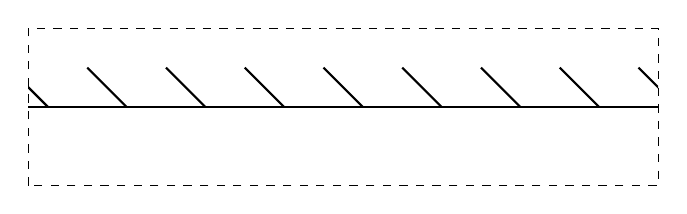
\begin{tikzpicture}[thick]
    \draw[dashed,thin] (0.25,-1) rectangle (8.25,1);
    \clip (0.25,-1) rectangle (8.25,1);
    \draw (-1,0) -- (9,0);
    \foreach \i in {0,1,...,8} {
      \draw (\i,.5) -- (.5+\i,0);
    }
  \end{tikzpicture}\\[10pt]
  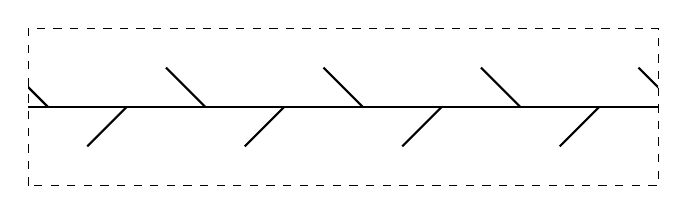
\begin{tikzpicture}[thick]
    \draw[dashed,thin] (0.25,-1) rectangle (8.25,1);
    \clip (0.25,-1) rectangle (8.25,1);
    \draw (-1,0) -- (9,0);
    \foreach \i in {0,2,...,8} {
      \draw (\i,.5) -- (.5+\i,0);
    }
    \foreach \i in {1,3,...,7} {
      \draw (\i,-.5) -- (.5+\i,0);
    }
  \end{tikzpicture}\\[10pt]
  \begin{tikzpicture}[thick]
    \draw[dashed,thin] (0.25,-1) rectangle (8.25,1);
    \clip (0.25,-1) rectangle (8.25,1);
    \draw (-1,0) -- (9,0);
    \foreach \i in {0,1,...,8} {
      \draw (\i,.5) -- (\i,0);
    }
  \end{tikzpicture}\\[10pt]
  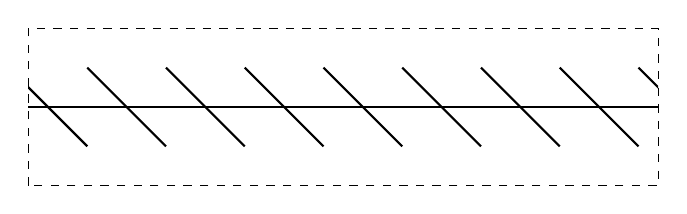
\begin{tikzpicture}[thick]
    \draw[dashed,thin] (0.25,-1) rectangle (8.25,1);
    \clip (0.25,-1) rectangle (8.25,1);
    \draw (-1,0) -- (9,0);
    \foreach \i in {0,1,...,8} {
      \draw (\i,.5) -- (1+\i,-.5);
    }
  \end{tikzpicture}\\[10pt]
  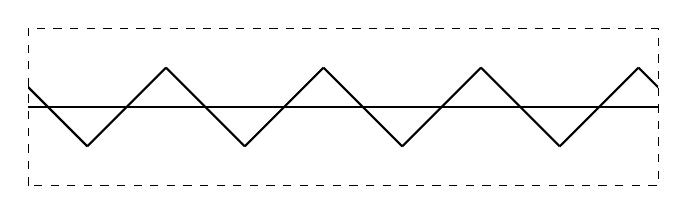
\begin{tikzpicture}[thick]
    \draw[dashed,thin] (0.25,-1) rectangle (8.25,1);
    \clip (0.25,-1) rectangle (8.25,1);
    \draw (-1,0) -- (9,0);
    \foreach \i in {0,2,...,8} {
      \draw (\i,.5) -- (1+\i,-.5);
    }
    \foreach \i in {1,3,...,7} {
      \draw (\i,-.5) -- (1+\i,.5);
    }
  \end{tikzpicture}\\[10pt]
  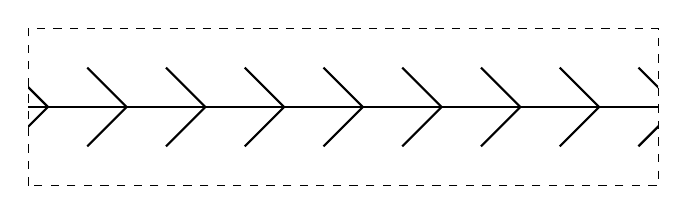
\begin{tikzpicture}[thick]
    \draw[dashed,thin] (0.25,-1) rectangle (8.25,1);
    \clip (0.25,-1) rectangle (8.25,1);
    \draw (-1,0) -- (9,0);
    \foreach \i in {0,1,...,8} {
      \draw (\i,.5) -- (.5+\i,0);
      \draw (\i,-.5) -- (.5+\i,0);
    }
  \end{tikzpicture}\\[10pt]
  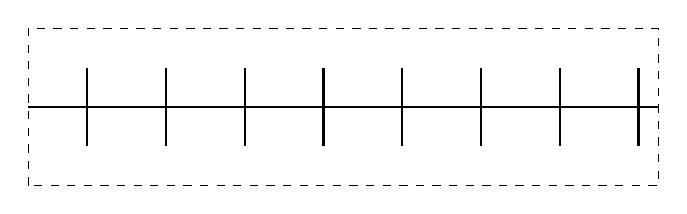
\begin{tikzpicture}[thick]
    \draw[dashed,thin] (0.25,-1) rectangle (8.25,1);
    \clip (0.25,-1) rectangle (8.25,1);
    \draw (-1,0) -- (9,0);
    \foreach \i in {0,1,...,8} {
      \draw (\i,.5) -- (\i,-.5);
    }
  \end{tikzpicture}

\end{center}

\section{Incidence geometries and the Levi graph}

\section{Affine geometry}
Barycentric calculus. Affine transformations. Euclidean / Hermitian geometry (isometries, conformity...)
\subsection{affine planes and Pappus' law}
\subsection{affine frames, affine planes}
\subsection{the affine group as an automorphism group}
\subsection{the affine group as a semidirect product}
\subsection{affine properties (parallelism, length ratios)}

\section{Inversive geometry (Möbius)}
\subsection{residue at a point is affine}
\subsection{Miquel's theorem}

\section{Projective geometry}
Projective spaces (projective invariance, cross ratio, harmonic range...). Conics/quadrics. (Classification in low dimensions?)
\par
complex algebraic plane projective curves (tangent complexes, singular points, polar, hessian, ...).
\subsection{projective planes}
\subsection{projective frames}
\subsection{the projective group and projectivities}
\subsection{projective properties (cross-ratio)}
\subsection{fundamental theorem of projective geometry}


% Local Variables:
% fill-column: 144
% latex-block-names: ("lemma" "theorem" "remark" "definition" "corollary" "fact" "properties" "conjecture" "proof" "question" "proposition" "exercise")
% TeX-master: "book"
% End:
